%%%% Header %%%%%%%%%%%%%%%%%%%%%%%%%%%%%%%%%%%%%%%%%%%%%%%%%%%%%%%%%%%%%%%%%%%

\documentclass[
  12pt
]{scrartcl}

\usepackage{jonas}

\bibliography{/home/jon/lucile/share/jowncloud/sci/refs/refs.bib}
\hyphenation{}

%%%% Meta data %%%%%%%%%%%%%%%%%%%%%%%%%%%%%%%%%%%%%%%%%%%%%%%%%%%%%%%%%%%%%%%%

\usepackage[
  pdfauthor   ={Jonas Schöley},
  pdftitle    ={The Gestational Age Pattern of Human Mortality},
  pdfsubject  ={},
  pdfkeywords ={},
  pdfproducer =Latex,
  pdfcreator  =pdflatex
]{hyperref}

\title{The Gestational Age Pattern of Human Mortality}
\author{Jonas Schöley\footnote{Max-Planck Odense Center on the Biodemography of Aging, University of Southern Denmark. Correspondence: \texttt{jschoeley@health.sdu.dk}.}}

%%%% Titlepage %%%%%%%%%%%%%%%%%%%%%%%%%%%%%%%%%%%%%%%%%%%%%%%%%%%%%%%%%%%%%%%%

\begin{document}

\maketitle

\thispagestyle{empty}

\begin{abstract}
\textsc{Abstract.} In order to check hypotheses about the cause for \enquote{ontogenescense} -- the phenomenon of a declining force of mortality prior to maturity -- I analyse data on human mortality by gestational age. Based on extensive microdata on births, fetal- and infant deaths in the US 2009 I calculate a joint fetal-infant lifetable by gestational age spanning week 23 until week 100 after the last menstrual period of the mother. This joint lifetable shows a remarkable regularity in the gestational age profile of fetal- and infant mortality: Mortality rates are declining over the whole observed age range with the exception of a \enquote{birth hump} peaking week 38. The absolute rate of decline slows down over age. This observed gestational age pattern of the force of mortality is consistent with three hypotheses concerning the causes for ontogenescense: 1) Adaptation: as the organism growths it becomes more resilient towards death, 2) transitional timing: the transition of birth is a stressful event and momentarily increases the force of mortality, 3) mortality selection: The frailest die first, resulting in the mean force of mortality to decline with age. In order to quantify the relative importance of these three processes I fit a three component mortality model against the observed force of mortality. The model describes the data with high accuracy, suggesting that the phenomenon of ontogenescense in humans is fully explained by the three hypotheses.
\end{abstract}

\clearpage

%%%% Text %%%%%%%%%%%%%%%%%%%%%%%%%%%%%%%%%%%%%%%%%%%%%%%%%%%%%%%%%%%%%%%%%%%%%

\section{Introduction} %%%%%%%%%%%%%%%%%%%%%%%%%%%%%%%%%%%%%%%%%%%%%%%%%%%%%%%%
\label{sec:introduction}

Biologists noticed that for humans and many other species the momentary risk of death decreases from birth until onset of maturity (\cite{Medawar1952}, see \cite{Levitis2011} for a comprehensive literature review). This phenomenon is called \enquote{ontogenescence} and various hypotheses have been put forward in an attempt to explain it (see \cite{Levitis2011} for an overview). The aim of this analysis is to check these hypotheses against data on human fetal- and infant mortality, ultimately seeking to explain the phenomenon of ontogenescence for humans.

Starting with the biological hypotheses on ontogenescense and using millions of individual level records on births, fetal- and infant deaths in the US I develop a mathematical model of early life mortality capable of answering questions like: How fast does a fetus/infant adapt to life? How risky is the transition of birth for the child? How important is mortality selection in explaining the aggregate age pattern of early life mortality? How heterogeneous is the fetal- population in terms of their mortality risk? Generally:

\begin{center}
  \emph{What drives the ontogenescent age decline of mortality?}
\end{center}

There are two levels of explanation: The individual and the population.\footnote{The following list of hypotheses is adapted from \cite{Levitis2011}. I added the distinction between individual level and population level hypotheses and selected a primary reference for each hypothesis based on Levitis literature review.}

\textsc{Individual:} The mortality decline over age represents growth, acquired robustness, adaptation\footnote{In this article I will use the term \enquote{adaptation} as referring to an individual adjusting to the outside world and thereby decreasing its mortality risk. I do not use the term on an evolutionary level.}, risk mitigation -- all taking place within an organism. Examples of individual level hypotheses are:
  \emph{Growth-trade-off:} The capability for fast growth is traded against higher mortality risks. The larger (older) the individual, the less need is there to make that trade-off (e.\,g.~\cite{Chu2008}).
  \emph{Robustness:} growth leads to robustness (e.\,g.~\cite{Munch2006}).
  \emph{Transitional timing:} as the organism grows it has to pass a series of critical transitions, potentially dying at each. These transitions are concentrated early in life and therefore the mortality risk is concentrated in early life (\cite{Levitis2011}).

\textsc{Population:} The mortality decline over age represents a selection effect: On average, the frailest individuals die first, the stronger individuals survive. Therefore, on the population level, the mean risk of death decreases over age. Examples of population level hypotheses are:
  \emph{Heterogeneous frailty:} the mortality decline over age represents a selection effect\footnote{Within this article I relate the term \enquote{selection} solely to mortality without any implications for inheritance of specific traits as would be implied by its Darwinian meaning.} -- on average, the frailest individuals die first, the stronger individuals survive. Therefore, on the population level, the mean risk of death decreases over age (e.\,g.~\cite{Vaupel1985}).
  \emph{Quality control:} the frailest die first, terminated by their kin (\cite{Hamilton1966}).

The questions of course is: Which of these hypotheses is suggested by the data for present day humans being born into a modern health care system?

\section{Data and Methods} %%%%%%%%%%%%%%%%%%%%%%%%%%%%%%%%%%%%%%%%%%%%%%%%%%%%
\label{sec:data_and_methods}

The vital statistics of the US (births, deaths) are designated for public use. The extent of the data is remarkable and facilitates detailed statistical analysis. I use about four million records on individual births, infant deaths and fetal deaths in the conception cohort 2009. This data is derived from the \enquote{US Birth Cohort Linked Birth - Infant Death Data Files} and the \enquote{Fetal Death Data Files} for the years 2009 and 2010 (\cite{DVS2015}). The fetal death file does \emph{not} include cases of induced abortions. Using the Kaplan-Meier estimator I produce a lifetable survival curve from this individual level data. Two separate lifetables are produced: 1) \emph{Infant mortality by day of age}, both sexes, US conception cohort 2009, from birth to 365 days after birth, and 2) \emph{joint fetal- and infant mortality by week of gestation}, both sexes, US conception cohort 2009, from week 23 to week 100 of gestation.

It might surprise that I choose to look at the gestational age pattern of joint fetal- and infant mortality in order to shed light on the underlying process of ontogenescense. The reasoning behind this move is manifold: As will be demonstrated, the gestational age pattern of mortality for fetal- and infant deaths shows a remarkable regularity which lends itself to statistical analysis. Furthermore, the theory on ontogenescense is not limited to the time after birth. In fact \textcite{Levitis2011} shows a rough estimate of daily human mortality rates from conception until the $12^{th}$ birthday in the context of discussing \enquote{the evolutionary demography of ontogenesis}. Therefore using only half of the available data (either on infant- or on fetal- deaths) would be an arbitrary limitation. Using gestational age instead of demographic age also has the advantage of making a major source of unobserved heterogeneity in early life mortality observable: The different gestational ages at birth.

The final model of the gestational age pattern of human mortality is informed by the theory on ontogenescense and by an exploratory analysis of human infant- and joint fetal-infant mortality. In a first step of analysis I plot the lifetable mortality rates for infants over age. The hypotheses on ontogenescense are checked against the observed mortality pattern in order to identify promising candidates. The same exercise is then repeated with the observed mortality pattern of the joint fetal-infant lifetable over gestational age. At the end of this explorative analysis it should be clear which hypotheses on ontogenescense to include in a mathematical model of the \emph{gestational age pattern of human mortality}. This model is then formulated and fitted against the lifetable mortality rates using Poisson-Maximum-Likelihood.

\section{The Age Pattern of Present US Infant Mortality} %%%%%%%%%%%%%%%%%%%%%%
\label{sec:the_daily_age_pattern_of_present_day_us_infant_mortality}

In order to see the true face of ontogenescence in the present day it is necessary to drill down to the daily age pattern of infant mortality (see figure \ref{fig:us_imort_2009_mx}).

\begin{figure}[!htb]
  \begin{subfigure}[t]{0.5\textwidth}
    \centering
    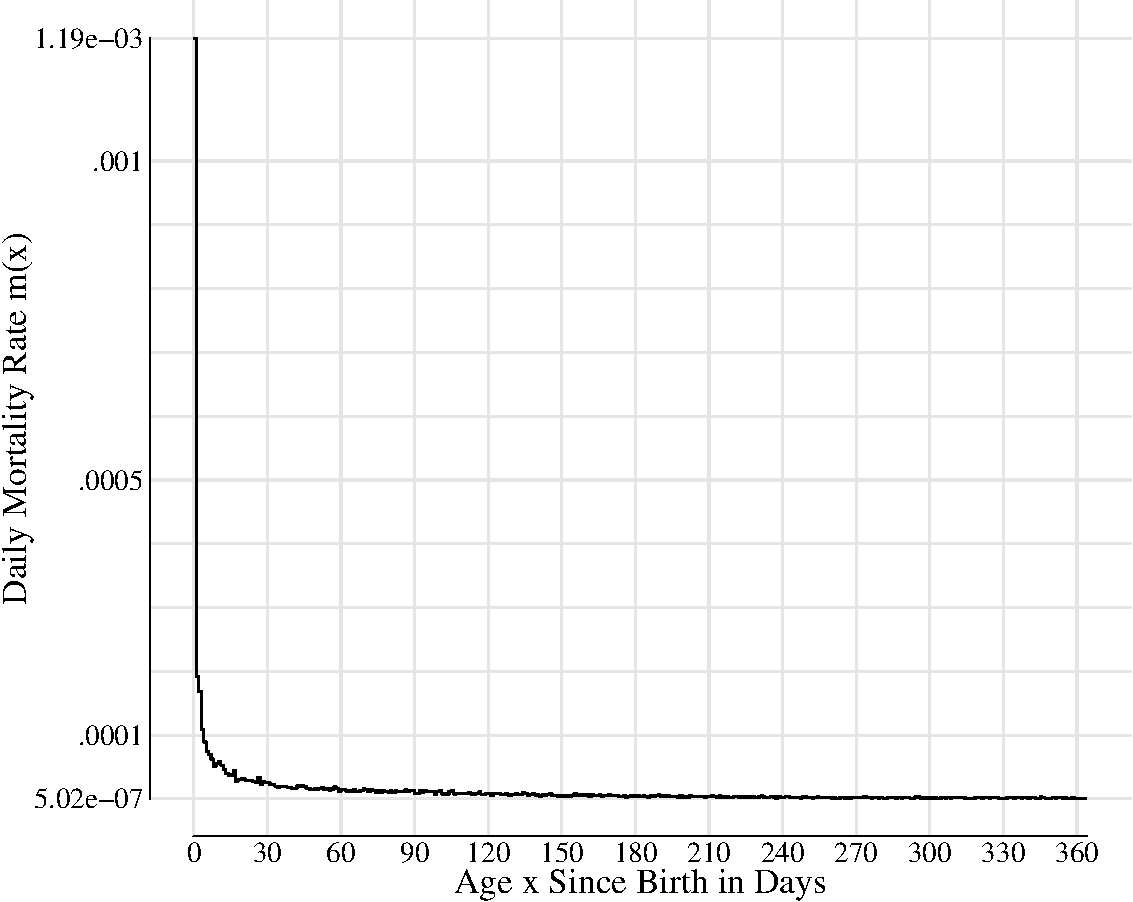
\includegraphics[width = \textwidth]{./fig/us_imort_2009_mx.pdf}
    \subcaption{Linear $y$-scale.}
    \label{fig:us_imort_2009_mx_a}
    \end{subfigure}%
  ~
    \begin{subfigure}[t]{0.5\textwidth}
    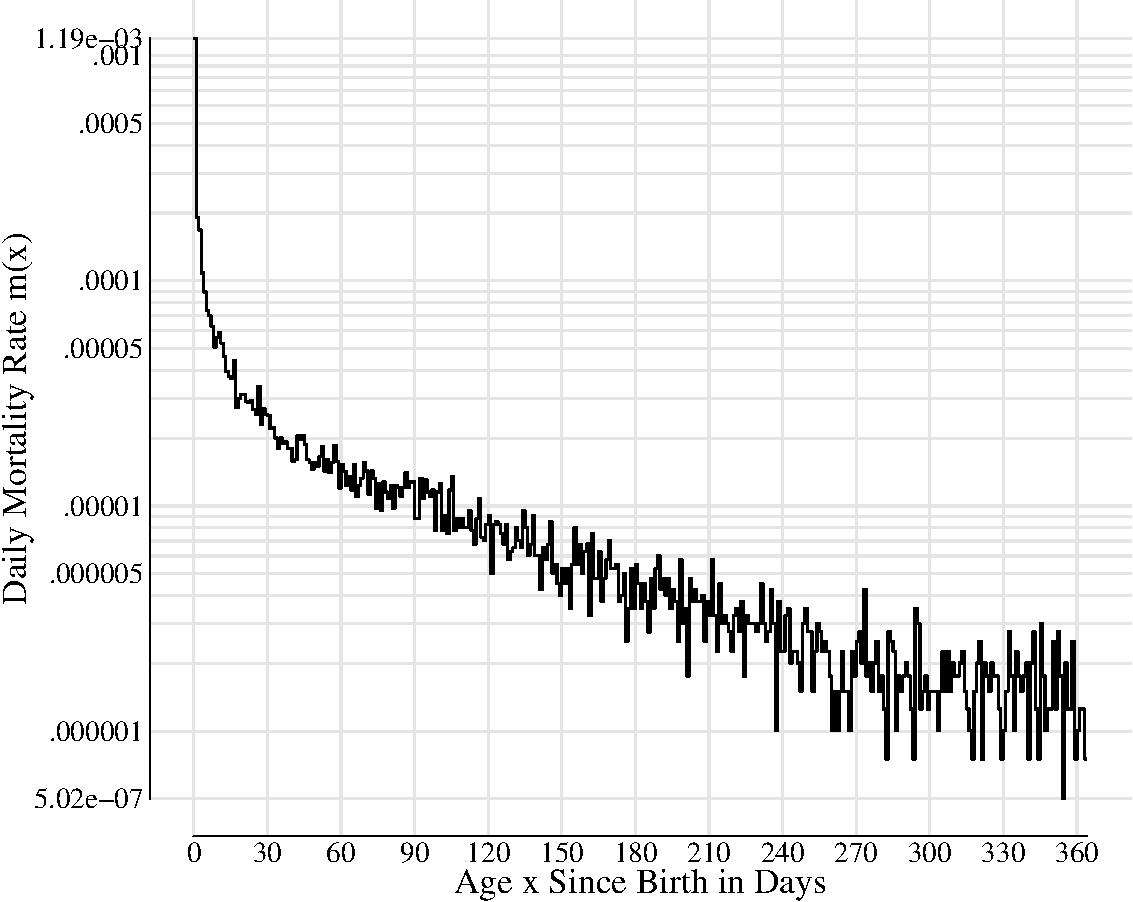
\includegraphics[width = \textwidth]{./fig/us_imort_2009_log_mx.pdf}
    \subcaption{Logarithmic $y$-scale.}
    \label{fig:us_imort_2009_mx_b}
    \end{subfigure}%
    \caption{The daily age pattern of infant mortality for US infants conceived in 2009. Individual level data source: \cite{DVS2015}.}
    \label{fig:us_imort_2009_mx}
\end{figure}

It is plain to see that the absolute majority of the infant mortality risk is concentrated at the day of birth (see figure \ref{fig:us_imort_2009_mx_a}). Of all observed infant deaths for the US conception cohort 2009, 25\,\% occur at the day of birth and nearly half of them within two weeks after birth. The infant mortality is clustered in the postpartum period. This is strong evidence for two hypotheses:
\begin{inparaenum}
  \item \emph{transitional timing:} Birth is a high risk transition and temporarily increases an individuals mortality risk.
  \item \emph{heterogeneity:} Birth is a strong selector and selects the frailest individuals out of the population.
\end{inparaenum}
While there are many possible sources for unobserved heterogeneity regarding the risk of death, a major contribution must be the heterogeneity in gestational ages at birth. Age is defined as time since birth. This definition is ignorant to the fact that infants are born at different times after conception. We know that mortality risk is highly dependent on the gestational age at birth. The lower the gestational age, the lower the ability to survive the transition of birth (e.\,g.~\cite{Lubchenco1972}). Therefore, in paediatric contexts, a different measure of time is used: The \emph{gestational age}, defined as weeks since the last manse.

Compressing these thoughts into a single sentence it can be hypothesized that \emph{birth gives shape to the age pattern of infant mortality by momentarily increasing the risk of death for every individual and by selecting the frailest individuals out of the population.}

While neonatal mortality seems to be dominated by the trauma of birth, what about mortality after the first month of age? Thanks to the tremendous success in reduction of infant mortality we rarely see deaths after the postpartum period in our data, yet we can still make out an age pattern: Starting at around 50 days of age the decline in infant mortality follows an exponential decay (as can be seen in figure \ref{fig:us_imort_2009_mx_b} as a log-linear decrease in mortality over age). This finding can be interpreted as a sign for \emph{adaptation}: The growth-rate of a child is the highest right after birth and declines from there on. If we assume that level of growth and level of mortality are inversely related, then the largest decline in mortality will fall into the period of the fastest growth, resulting in a negative exponential form of mortality decline due to growth/adaptation.\footnote{The negative exponential shape of infant mortality is famously specified in the Siler model (\cite{Siler1979}).}

On the basis of the above ideas we hypothesize that infant mortality can be explained as the sum of three components:
\begin{compactenum}
  \item The exponential decrease of mortality after 50 days of age is explained by \emph{adaptation} -- robustness acquired with growth,
  \item the mortality outlier at the day of birth is explained by \emph{transitional timing} -- the added stress due to the struggle of birth, and
  \item the super-exponential decrease of mortality right after birth is explained by \emph{selection} against the most frail.
\end{compactenum}

\section{The Gestational Age Pattern of US Mortality} %%%%%%%%%%%%%%%%%%%%%%%%%
\label{sec:the_gestational_age_transformation}

From a statistical point of view, the clustering of the majority of mortality risk in a single data point is problematic. We can not learn much about the age pattern of infant mortality and of its components if the bulk of the variability is contained between two points: day 0 and day 1 after birth. Therefore I propose to look at mortality across the \emph{gestational age scale}. This scale transformation changes interpretation and shape of the mortality data in advantageous ways: Different gestational ages at birth are eliminated as a source of unobserved heterogeneity and the risky transition of birth is distributed along the time axis instead of clustered at the start. Because most fetal deaths occurring during the first half of the pregnancy are undetected and/or unreported we condition our population upon surviving to the $23^{rd}$ week of gestational age. From then on the vast majority of fetal deaths are believed to be registered in the US.

The human gestational age pattern as seen on our data has a very distinctive shape (see figure \ref{fig:us_fimort_2009_mx}). Mortality is highest at the start of the observation window and continuously decreases with a declining rate of change until the end of observation, only to be disrupted by a \emph{\enquote{birth hump}}. It seems that the \emph{birth spike} we can observe in infant mortality over age spread out into a distribution closely following the distribution of gestational ages at onset of labour. This can be explained on the population level: The higher the probability of birth at a given gestational age $x$, the higher the contribution of the stress at birth to the population hazard.

Overall, the data is consistent with what we see in infant mortality and the \emph{adaptation}, \emph{transitional timing} and \emph{selection} hypothesis continue being sensible choices for a final model.

\begin{figure}[!htb]
  \centering
  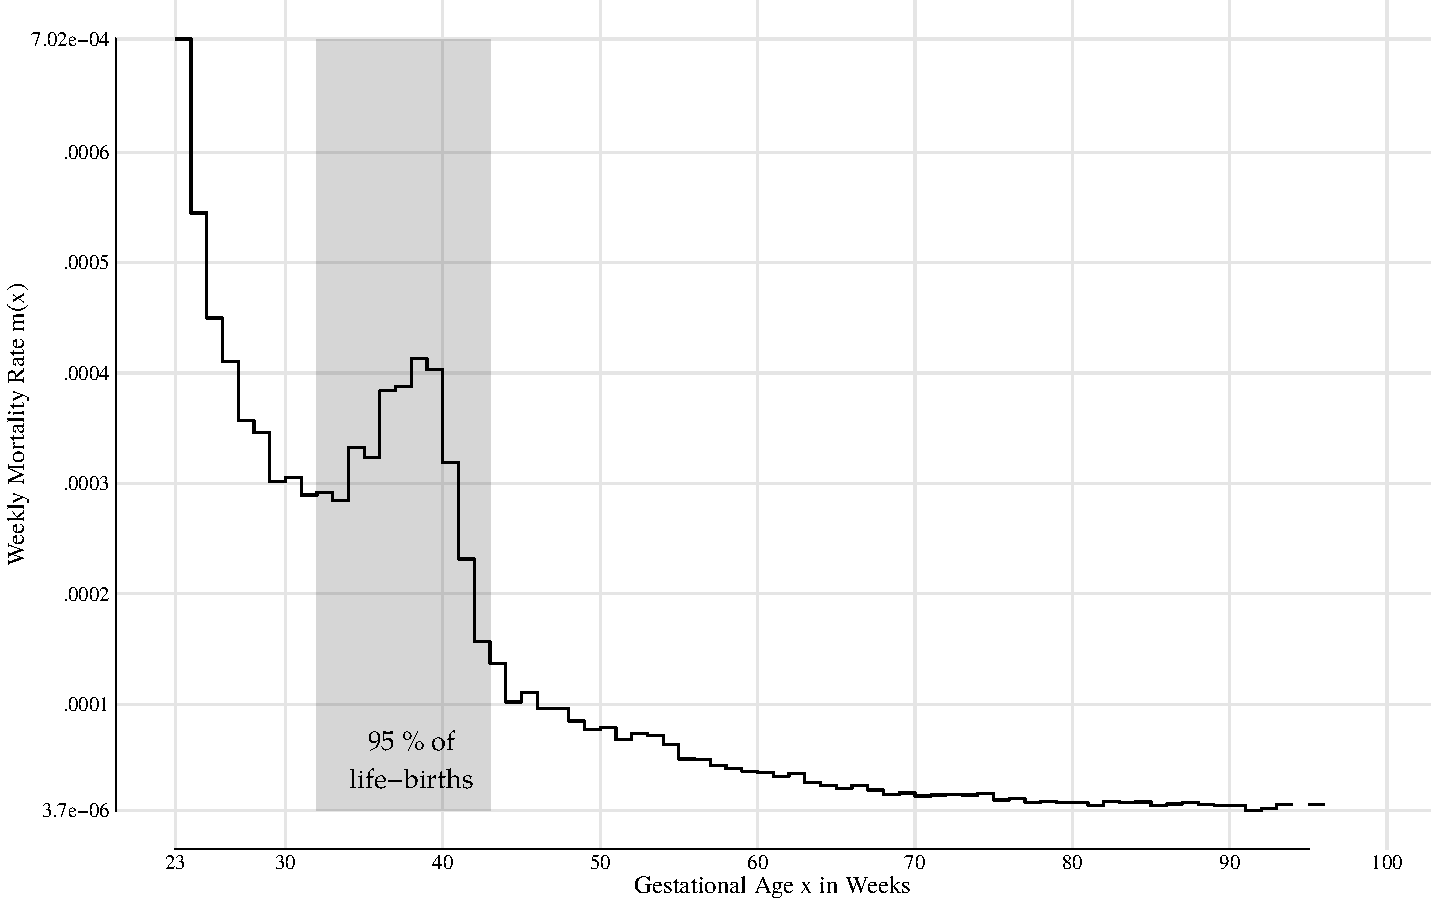
\includegraphics[width = \textwidth]{./fig/us_fimort_2009_mx.pdf}
  \caption{The gestational age pattern of human mortality for US fetus and infants conceived in 2009. Individual level data source: \cite{DVS2015}.}
  \label{fig:us_fimort_2009_mx}
\end{figure}

\section{A Model of Gestational Age Mortality} %%%%%%%%%%%%%%%%%%%%%%%%%%%%%%%%
\label{sec:modelling_the_gestational_age_pattern_of_human_mortality}

We identified three explanations for the decreasing age pattern in infant mortality which make sense in light of the available data:
\begin{inparaenum}
  \item \emph{Adaptation} as robustness acquired with growth,
  \item \emph{transitional timing} as the added stress due to the struggle of birth, and
  \item \emph{selection} as the early death of the frailest.
\end{inparaenum}
This can be expressed in the following functional form:

$$
  \underbrace{
    \overline{\mu}(x)
  }_{\substack{
    \text{Population hazard}\\ \text{at gestational age}~x
  }} =
  \underbrace{
    E[Z(x)]
  }_{\substack{
    \text{Average frailty}\\ \text{in population}\\ \text{at gestational age}~x
  }} \times
  \underbrace{
    \alpha_1 e^{-\lambda x}
  }_{\substack{
    \text{Adaptation component}\\ \text{of hazard}\\ \text{at gestational age}~x
  }} +
  \underbrace{
    \alpha_2 b(x)
  }_{\substack{
    \text{Birth trauma component}\\ \text{of hazard}\\ \text{at gestational age}~x.
  }}
$$

Assuming the frailty to be initially Gamma-distributed with a unity mean the adaptation component and the average frailty translate into the well known Gamma-Gompertz model. Therefore,

$$
  E[Z(x)] \times \alpha_1 e^{-\lambda x} = \frac {\alpha_1 e^{-\lambda x}} {\frac{\gamma \alpha_1} {-\lambda} (e^{-\lambda x} - 1) + 1},
$$

where $\gamma$ is the variance of the frailties in the population at the beginning of observation.\footnote{See \cite{Vaupel1979} for the original formulation of the (Gamma) frailty model; see \cite{Vaupel1985} for the potential application of frailty models to infant mortality; see \cite{Vaupel2014} for a recent discussion of the Gamma-Gompertz model; see \cite{Wienke2011} for a general introduction to frailty models; see \cite{Wienke2003} for an application of the Gamma-Gompertz model.}

The distribution of gestational ages at onset of labour $b(x)$ is skewed to the left and truncated to the right with a mode at around a gestational age of 40 weeks. While preterm deliveries can stretch into the second trimester of pregnancy, labour is usually induced at postterm (>42 weeks of gestation). The scaled Beta distribution has the required features to model this situation. It is \emph{continuous}, can be \emph{left tailed}, and can be scaled over an arbitrary domain (in our case week 23 until week 47 -- the week of the last registered delivery in the data). The distribution of the gestational age at onset of labour has the following form,

$$
b(x) = \frac{1}{B(s_1,s_2)} \times \frac{(x-23)^{s_1-1}\cdot(47-x)^{s_2-1}} {(47-23)^{s_1+s_2-1}},
$$

with $B(s_1,s_2)$ being the Beta function. The complete model has the 6 free parameters:

\begin{tabular}{ll}
  $\alpha_1$ & The initial mortality level (at week 23 and process time 0). \\
  $\lambda$ & The relative rate of mortality decline (adaptation). \\
  $\gamma$ & The initial variance of frailties (at week 23 and process time 0) \\
  $\alpha_2$ & The overall added mortality risk due to the stress of birth. \\
  $s_1$ & The modal gestational age at onset of labour (in weeks after week 23). \\
  $s_2$ & The shape of the age distribution at onset of labour. \\
\end{tabular}

Estimating the model on the joint fetal-infant lifetable for the US conception cohort of 2009 yields a close fit with sensible parameter estimates (see figure \ref{fig:us_fimort_2009_mx_predobs}).

\begin{figure}[!htb]
  \centering
  \includegraphics[width = \textwidth]{./fig/us_fimort_2009_mx_predobs.pdf}
  \caption{The gestational age pattern of human mortality for US fetus and infants conceived in 2009. Lifetable mortality rates versus predicted hazard. Individual level data source: \cite{DVS2015}.}
  \label{fig:us_fimort_2009_mx_predobs}
\end{figure}

\clearpage

%%%% Bibliography %%%%%%%%%%%%%%%%%%%%%%%%%%%%%%%%%%%%%%%%%%%%%%%%%%%%%%%%%%%%%

\sloppy
\printbibliography

%\clearpage

%%%% Appendix %%%%%%%%%%%%%%%%%%%%%%%%%%%%%%%%%%%%%%%%%%%%%%%%%%%%%%%%%%%%%%%%%

% appendix figures follow A1, A2, B1... scheme
%\renewcommand\thefigure{\thesection.\arabic{figure}}
%\setcounter{figure}{0}

%\begin{appendix}
%\end{appendix}

\end{document}